\documentclass[12pt, a4paper]{article}
\usepackage[a4paper, includeheadfoot, mag=1000, left=2cm, right=1.5cm, top=1.5cm, bottom=1.5cm, headsep=0.8cm, footskip=0.8cm]{geometry}
% Fonts
\usepackage{fontspec, unicode-math}
\setmainfont[Ligatures=TeX]{CMU Serif}
\setmonofont{CMU Typewriter Text}
\usepackage[english, russian]{babel}
% Indent first paragraph
\usepackage{indentfirst}
\setlength{\parskip}{5pt}
% Diagrams
\usepackage{graphicx}
\usepackage{float}
% Page headings
\usepackage{fancyhdr}
\pagestyle{fancy}
\renewcommand{\headrulewidth}{0pt}
\setlength{\headheight}{16pt}
%\newfontfamily\namefont[Scale=1.2]{Gloria Hallelujah}
\fancyhead{}

\usepackage{amsmath}

\graphicspath{ {./images/} }

\usepackage{listings}
\lstdefinestyle{lablisting}{
  basicstyle=\scriptsize\ttfamily,
  numbers=left,
  stepnumber=1,
  otherkeywords={EOF, O\_RDONLY, STDIN\_FILENO, STDOUT\_FILENO, STDERR\_FILENO},
  numbersep=10pt,
  showspaces=false,
  showstringspaces=false
}

\newcommand{\specialcell}[2][l]{%
  \begin{tabular}[#1]{@{}l@{}}#2\end{tabular}}

\begin{document}

% Title page
\begin{titlepage}
\begin{center}

\textsc{Федеральное государственное автономное образовательное учреждение высшего\\
образования "Национальный исследовательский университет ИТМО"}
\vfill
\textbf{Лабораторная работа №1\\[4mm]
по дисципение "Информационная безопасность"\\[4mm]
Атака на алгоритм шифрования RSA посредством метода Ферма\\[4mm]
}
\textit{Вариант 10\\[20mm]}
\begin{flushright}
Выполнил: студент Саржевский И.А.
\\[2mm]Группа: P3402\\[4mm]
Преподаватель: к.т.н., доцент\\
Маркина Т.А.
\end{flushright}
\vfill
г. Санкт-Петербург\\[2mm]
2021 г.

\end{center}
\end{titlepage}

\begin{huge}Лабораторная работа №1\end{huge}\\[4mm]
\begin{Large}Атака на алгоритм шифрования RSA посредством метода\\Ферма\end{Large}\\

\section*{Цель работы}

Изучить атаку на алгоритм шифрования RSA посредством метода Ферма.

\section*{Задание}

Алгоритм шифрования RSA состоит из следующих шагов:

\begin{enumerate}
  \item Выбираются простые числа p и q, вычисляется n = p * q;
  \item $\phi(n) = (p - 1)(q - 1)$;
  \item Находится число e, взаимно простое $\phi(n)$;
  \item Вычисляется $d$, такое, что $de$ эквивалентно единице по модулю $\phi(n)$.
\end{enumerate}

$(n,e)$ - публичный ключ. Для шифрования сообщение разбивается на блоки $t (<n)$,
зашифрованный текст: $c = t^e\:mod\:n$.

Для дешифрования используется приватный ключ $(n,d)$: $t = c^d\:mod\:n$.

В данной лабораторной работе рассматривается атака с помощью метода Ферма. Он
заключается в решении уравнения $t^2 - w^2 = n$, иными словами, поиске $t$, при
котором $t^2 - n$ - простое число. Поиск начинается с $\sqrt{n}$, так как это
минимальное значение, при котором $t^2 - n \ge 0$. Затем текущее значение
инкрементируется на каждой итерации, производится поиск значения, при котором
$\sqrt{t^2 - n}$ является целым числом $w$. В таком случае\\$p = t + w; q = t - w$,
зная которые можно расшифровать текст.

Разработанная программа принимает путь к yaml-файлу, в котором описаны исходные
данные: N, e и блоки данных C.
\newpage
\section*{Исходные данные}

\lstinputlisting[style=lablisting]{../src/var10.yaml}

\section*{Листинг разработанной программы}

\subsubsection*{main.rs}

\lstinputlisting[style=lablisting]{../src/main.rs}

\subsubsection*{rsa.rs}

\lstinputlisting[style=lablisting]{../src/rsa.rs}

\section*{Результаты работы программы}

\begin{figure}[H]
    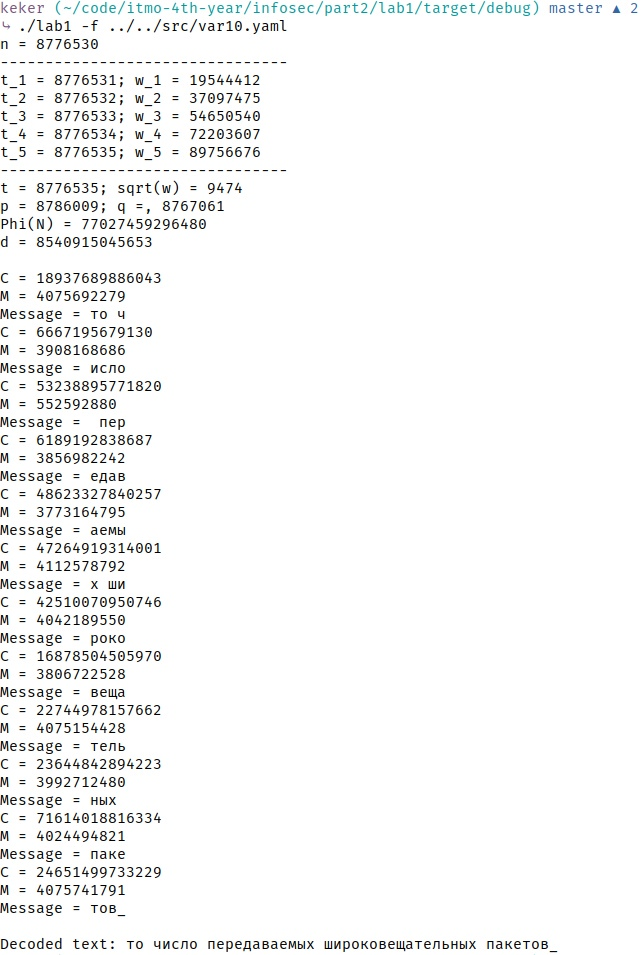
\includegraphics[scale = 0.5]{res}
    \caption{Результат работы программы}
    \centering
\end{figure}

\section*{Вывод}

В результате выполнения данной лабораторной работы была изучена атака на
алгоритм шифрования RSA методом Ферма. Была реализована программа, позволяющая
найти секретный ключ и расшифровать сообщение, зашифрованное с помощью RSA.

\end{document}
